\chapter{Introducción}\label{ch:introduccion}
\thispagestyle{empty}

\vspace{50pt}

\begin{adjustwidth}{50pt}{50pt}
    TODO
\end{adjustwidth}

\clearpage
\newpage
\thispagestyle{empty}
\mbox{}
\newpage

% Copyright (c) 2024, Francisco Fernandez
% License: CC BY-SA 4.0
%   https://github.com/fernandezfran/thesis/blob/main/LICENSE
\section{Contextualización}

El calentamiento global aparece como el mayor problema ambiental de este siglo.
El mismo se refiere al aumento de la temperatura media de la atmósfera y por 
ende a sus consecuencias en  el clima. Esto es debido al efecto que producen 
las actividades humanas, 
como por ejemplo la quema de combustibles fósiles, que emite 
a la atmósfera grandes cantidades de CO$_2$, entre otros gases de efecto 
invernadero, o la deforestación. Estos gases absorben la radiación infrarroja emitida por la tierra y la reemiten, 
provocando un incremento de la temperatura de la misma que lleva asociado un 
aumento en la frecuencia y la intensidad de eventos climáticos extremos. %\cite{houghton2005}. 
De acuerdo a el Panel Intergubernamental del Cambio Climático 
\cite{IPCC}, desde la época preindustrial, las actividades humanas han provocado 
aproximadamente 1.0$^{\circ}$C de calentamiento global y al ritmo actual se van 
a sobrepasar los 1.5$^{\circ}$C antes del 2050, un cambio en la temperatura
media que las medidas previas al aumento de las actividades mencionadas no habían llegado a alcanzar. Limitar el 
calentamiento a esta temperatura requiere que se realicen rápidamente cambios 
sin precedentes en la tecnología y en el comportamiento humano. Uno de los 
cambios más importante es el de la matriz energética, en la cual las energías 
renovables deberán suministrar alrededor del 80\% de la energía para 2050, donde 
los vectores energéticos, como las baterías de litio, juegan un rol fundamental 
debido a la intermitencia de estas formas de generación de energía.

El litio es el metal más liviano de la tabla periódica y uno de los elementos más
importantes dentro de los minerales necesarios en la producción de baterías de
litio. En particular, para la Argentina tiene un interés económico, social, 
industrial y tecnológico ya que es uno de los países que integran, junto a 
Bolivia y Chile, el Triangulo de Litio, el cual acumula el 70\% de las reservas 
mundiales de fácil extracción de este mineral. Esto último debido a que esta cantidad de reservas
se encuentran en salares de los que, a grandes rasgos, es más barato
extraer litio de ellos en comparación a las rocas de las cuales se puede extraer 
litio en una míneria usual, como las pegmatitas. A pesar de esto se tienen que
llevar a cabo distintas consideraciones ambientales, sociales y legales del 
proceso de extracción e incentivar el desarrollo de valor agregado a dicha 
extracción \cite{gutierrez2022, petavratzi2022, obaya2021, romero2021, 
heredia2020, fornillo2019}.

En esta tesis se presentan estudios computacionales sobre materiales para el 
desarrollo de electrodos de baterías de ion-litio de próxima generación. Se 
abordan dos perspectivas, una con el objetivo de tener baterías que frente a una 
carga rápida retengan un porcentaje considerable de la capacidad y otra 
utilizando electrodos que permitan almacenar mayor cantidad de energía que los 
actuales.


Las otras aplicaciones de la Figura \ref{fig:iea-Li} incluyen dispositivos
electrónicos, medicamentos, lubricantes, entre otras \cite{IEA}.

\say{Sin embargo} el litio representa el 7 \% de la demanda de minerales críticos
para vehículos eléctricos mientras que para almacenamiento en la red el porcentaje
se encuentra en el 10 \%. El resto del porcentaje de la demanda está abarcado por 
otros metales y minerales críticos, tales como grafito, cobre, níquel, manganeso, 
cobalto y silicio \cite{IEA}.

\begin{figure}[h!]
    \centering
    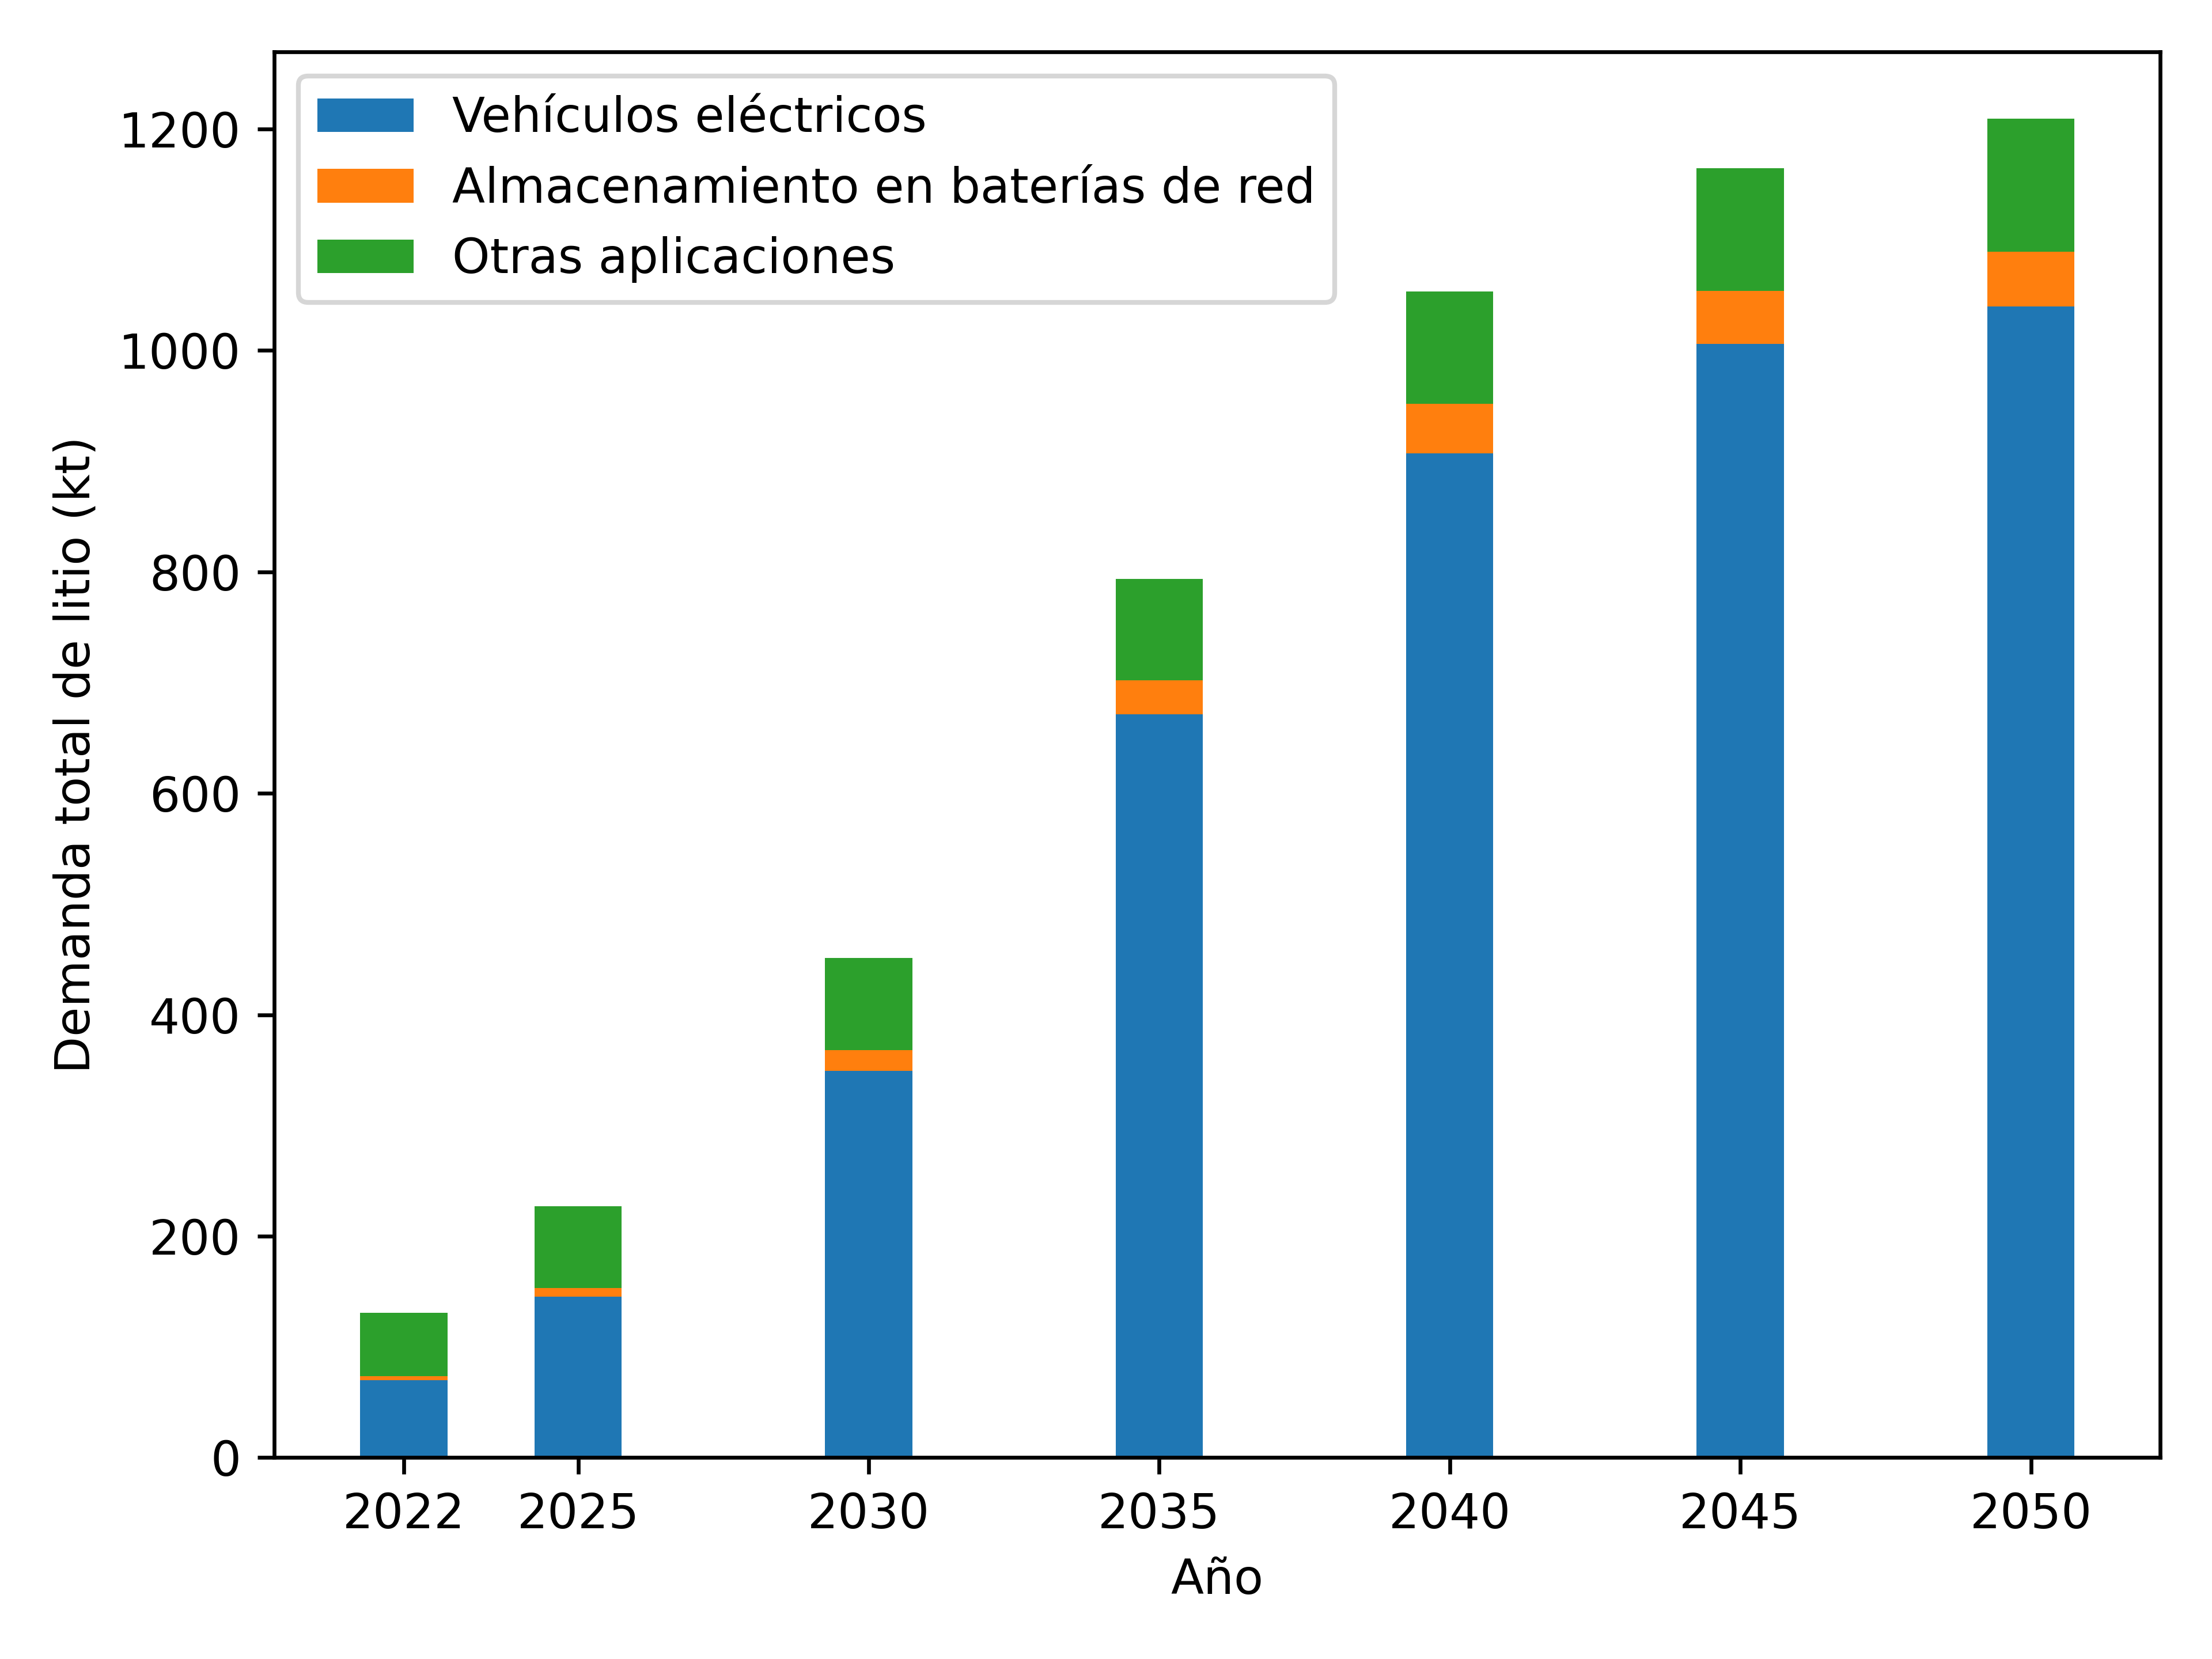
\includegraphics[width=.8\textwidth]{Introduccion/iea-Li.png}
    \caption{Proyección de la demanda total de litio en kilotoneladas por año y 
    aplicación. Fuente: \cite{IEA}.}
    \label{fig:iea-Li}
\end{figure}

\begin{figure}[h!]
    \centering
    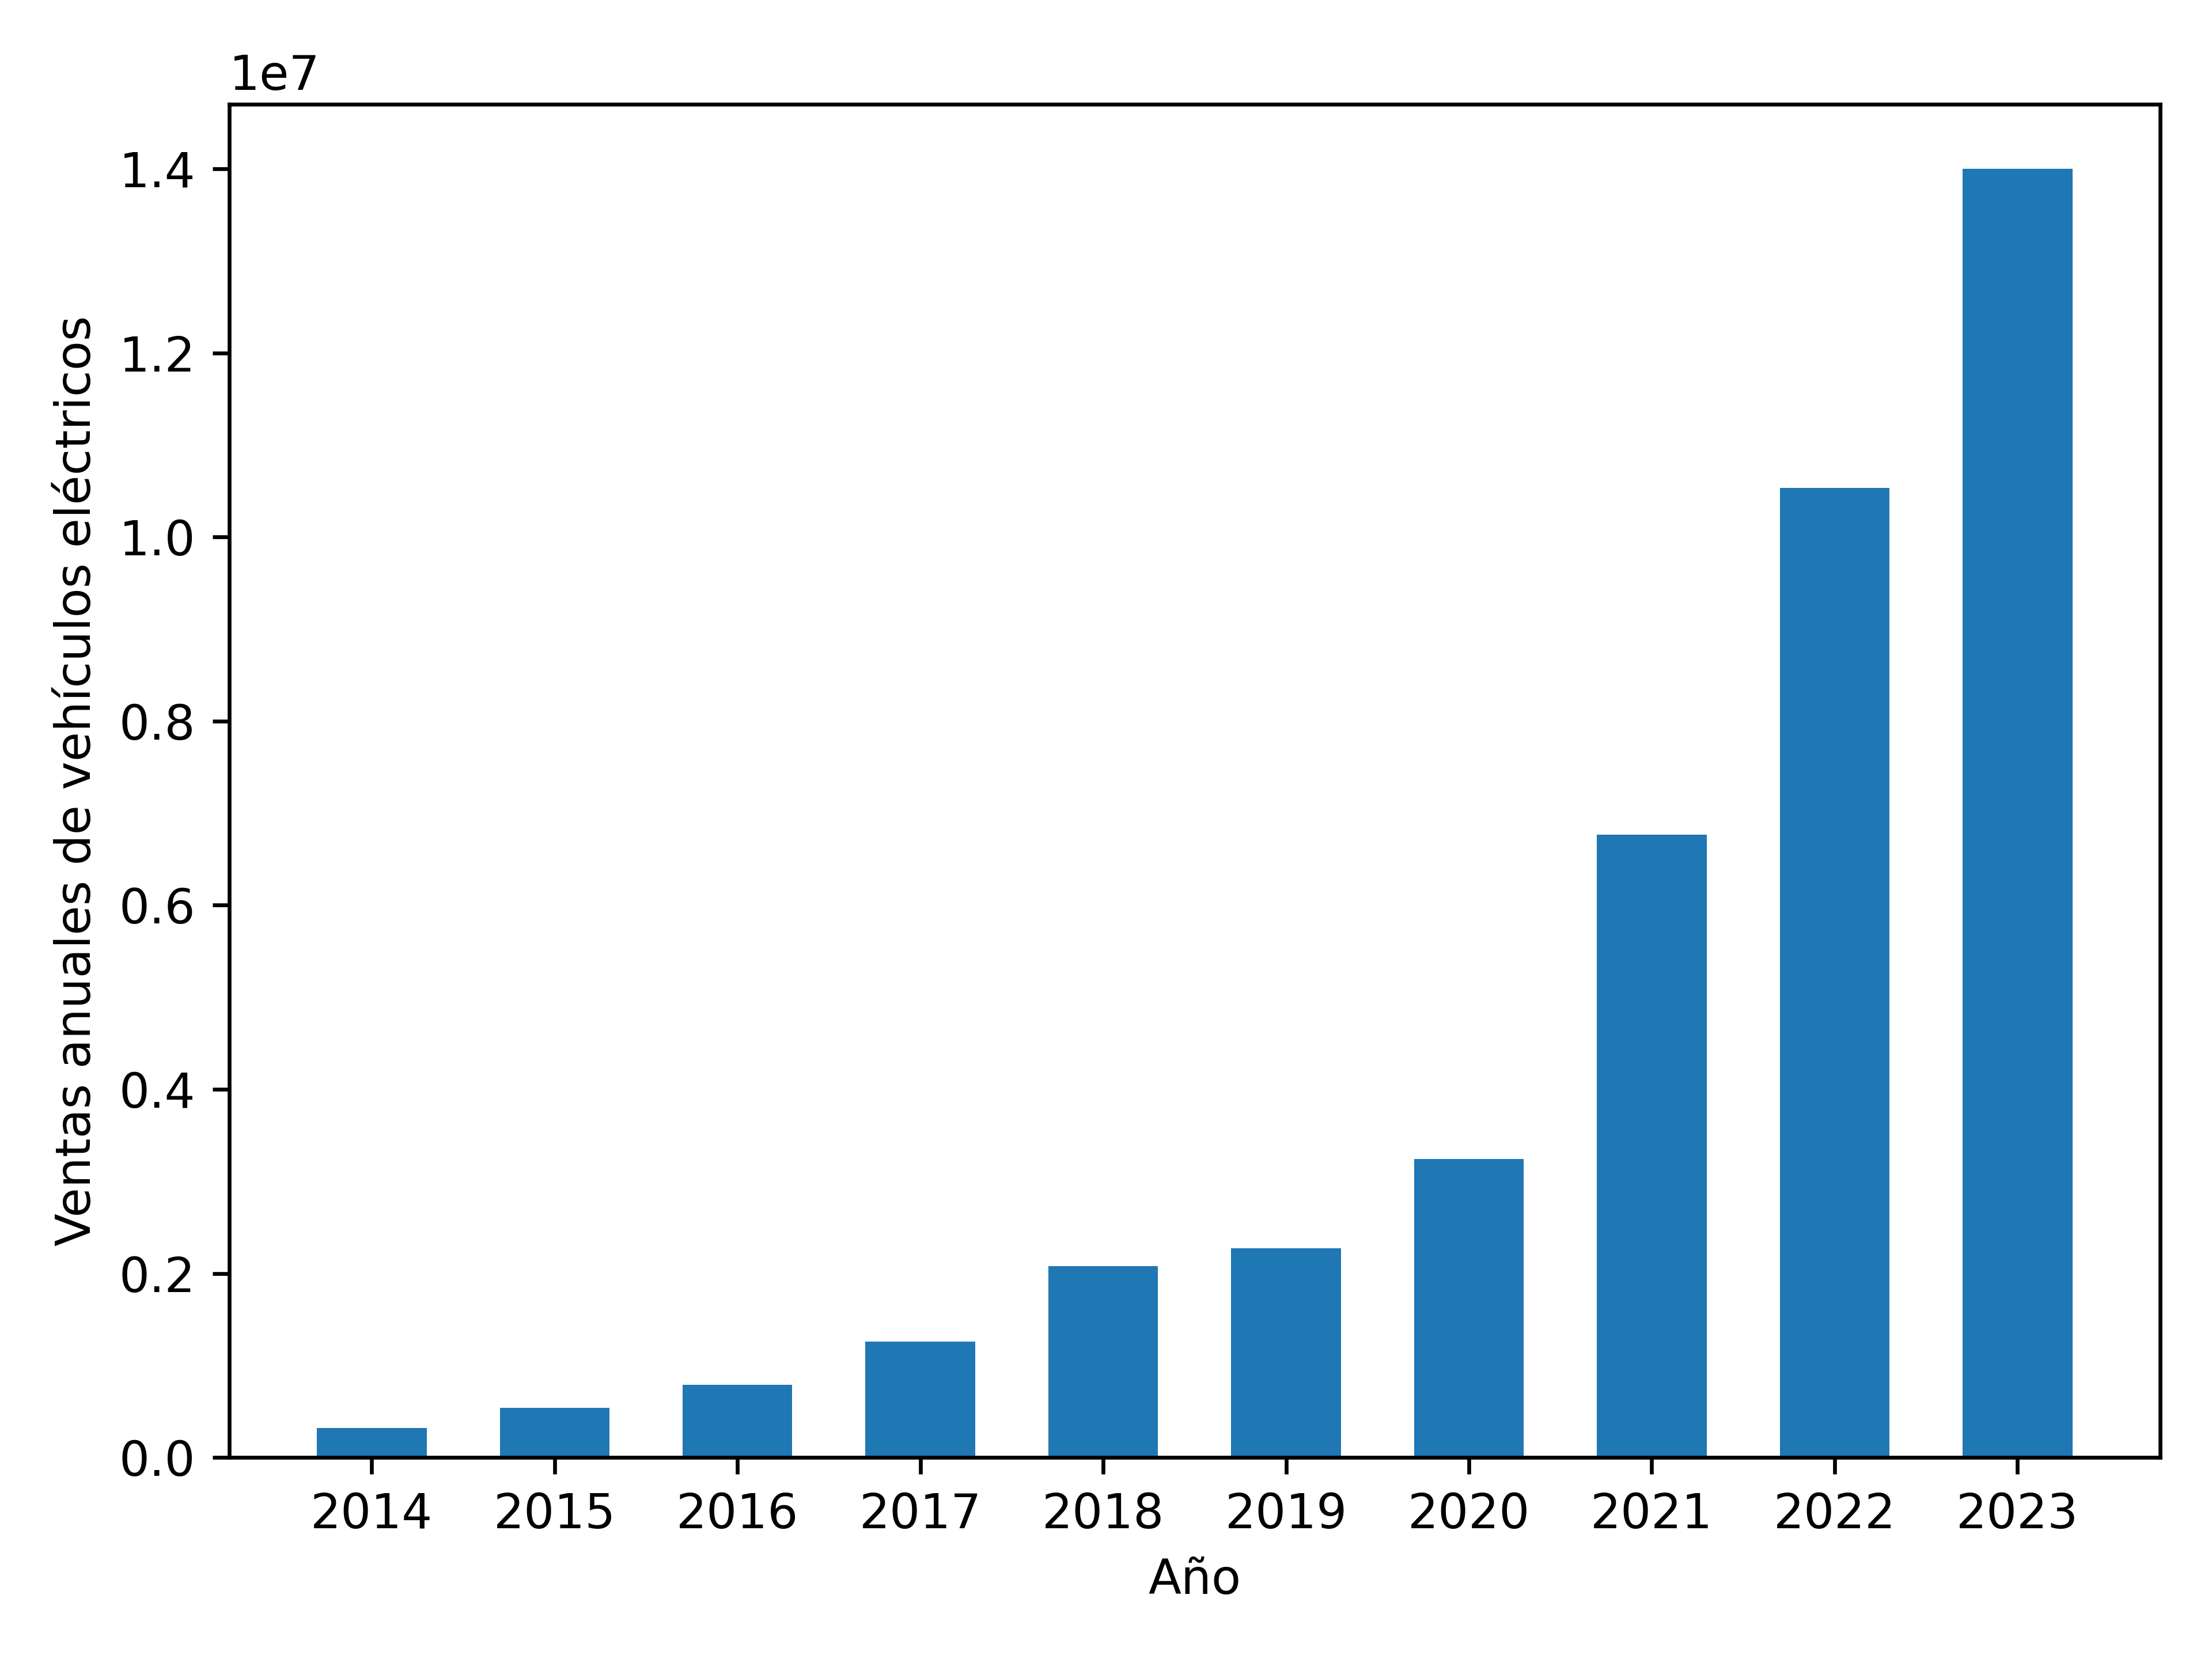
\includegraphics[width=.8\textwidth]{Introduccion/ev-volumes.png}
    \caption{Ventas anuales de vehículos eléctricos en la última década. Se 
    proyecta que para el 2030 las ventas asciendan a las 40 millones de unidades.
    Fuente: \cite{EVV}.}
    \label{fig:ev-volumes}
\end{figure}

\begin{figure}[h!]
    \centering
    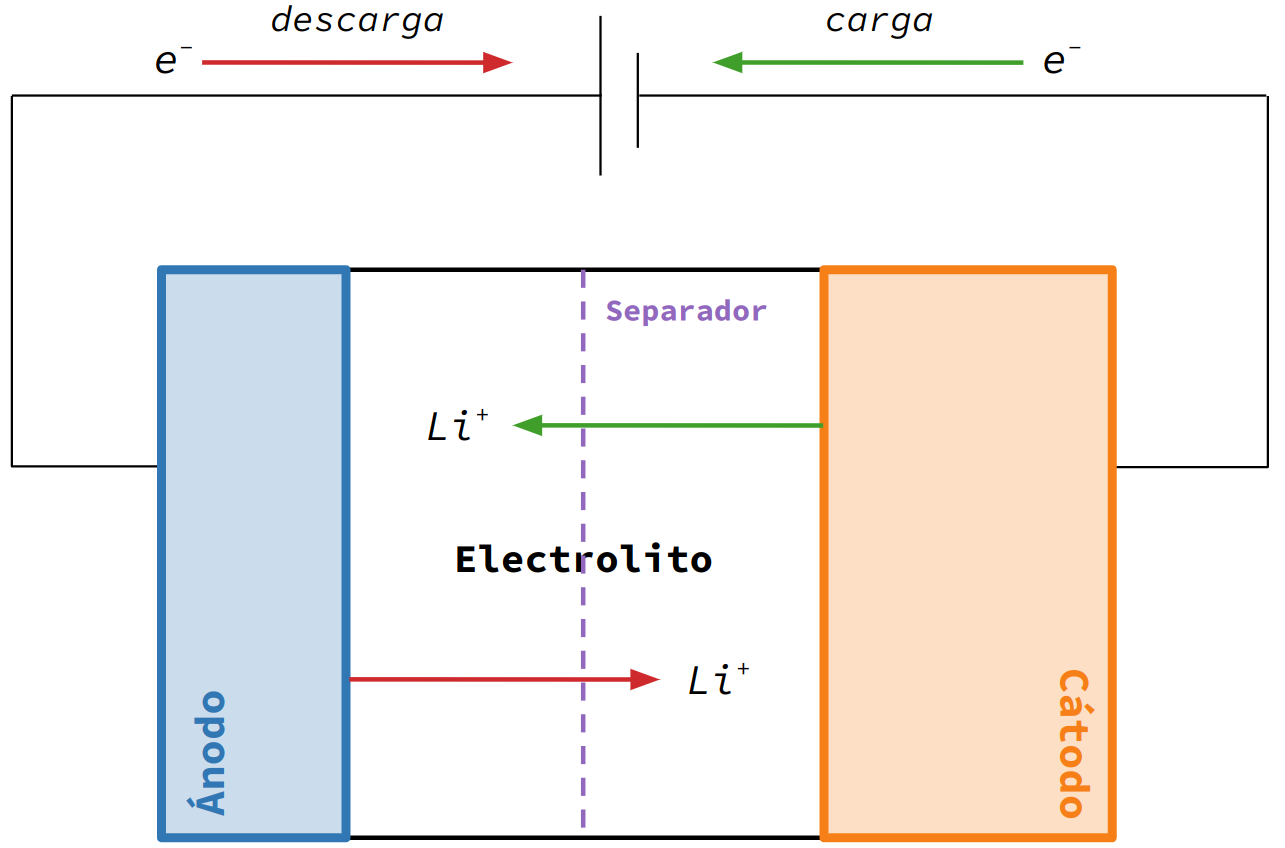
\includegraphics[width=.8\textwidth]{Introduccion/esquema_bateria.png}
    \caption{Esquema de las componentes y el funcionamiento de una batería de 
    ion-litio.}
    \label{fig:esquema-bateria}
\end{figure}
